\section{Zur Programmierung verwendete Software}
Auch wenn die Entwicklungsumgebung \textit{PlatformIO} in einer Variation von Editoren zur Verfügung steht, wird im Folgenden nur auf die 
Installation in \textit{Visual Studio Code} eingegangen.

\subsection{Visual Studio Code}
\href{https://code.visualstudio.com/}{Visual Studio Code Webseite}
\begin{figure}[h]
	\centering
	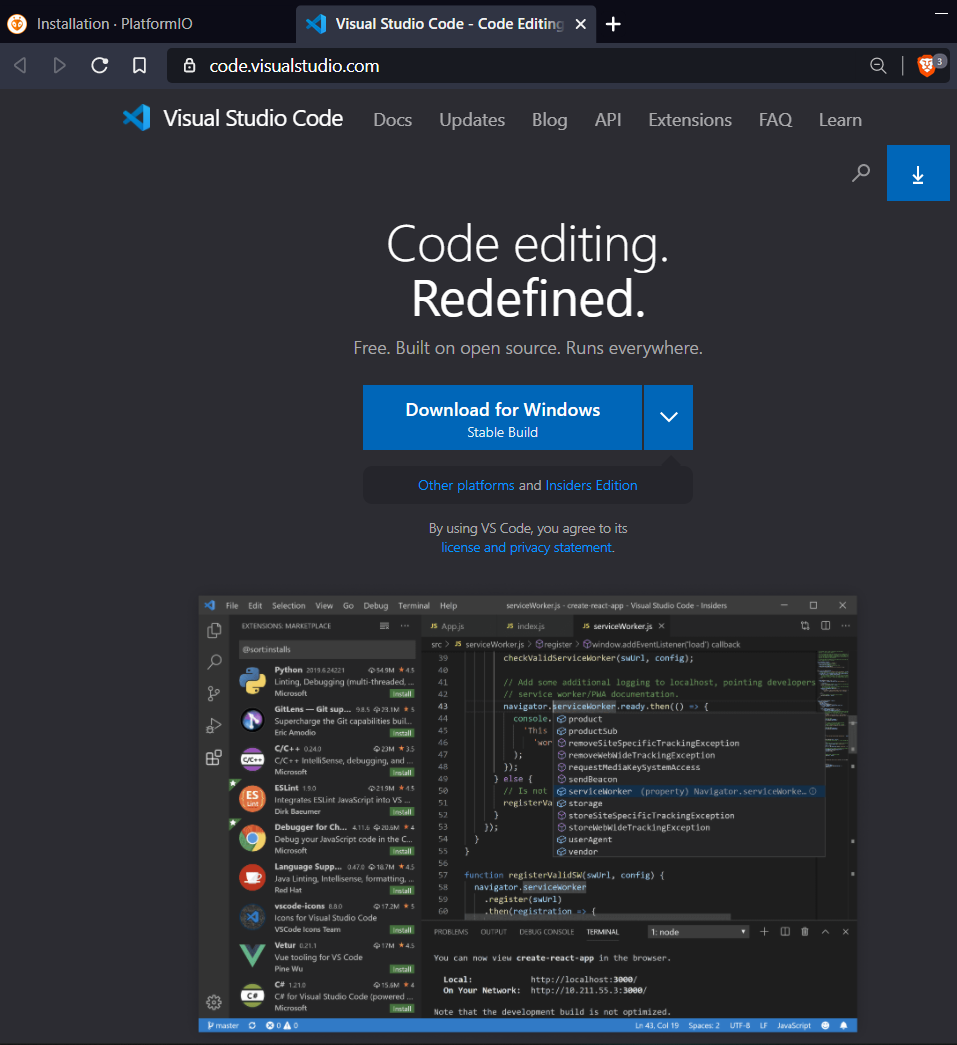
\includegraphics[width=0.8\textwidth]{bilder/Webseite_VSCode.png}
	\caption{Visual Studio Code Webseite}
\end{figure}

Visual Studio Code wird anschließend mit seiner Standard-Auswahl bei allen Abfragen installiert, weswegen hier auf eine genauere Dokumentation verzichtet wurde.

\subsection{PlatformIO IDE}
Hierbei handelt es sich um eine Erweiterung, welche mittels folgender Abbildung in Visual Studio Code installiert werden kann.\\
\href{https://platformio.org/install/ide?install=vscode}{PlatformIO Download Webseite}
\begin{figure}[h]
	\centering
	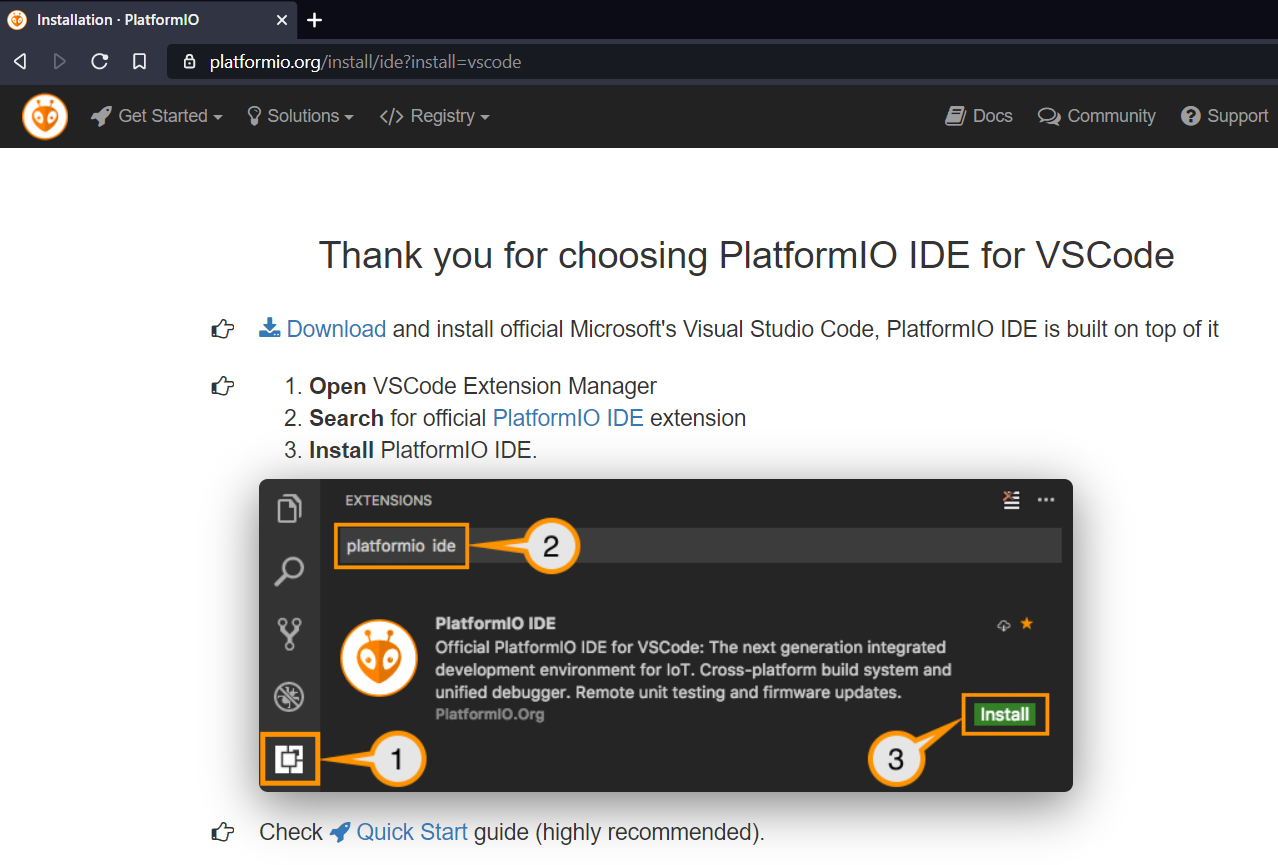
\includegraphics[width=0.8\textwidth]{bilder/Webseite_PlatformIO.png}
	\caption{PlatformIO Webseite}
\end{figure}

\textbf{Anmerkung:}\\
In neueren Versionen von Visual Studio Code ist das Icon des \textit{Extension Managers} nicht mehr das in obiger Abbildung gezeigte, sondern folgendes:

\includegraphics[align=t,width=0.8cm]{bilder/Icon_Extension_Manager.png}\\

Dieser Vorgang kann einige Minuten in Anspruch nehmen, und sollte am Ende zu einem \textit{Reload Window} auffordern. Danach ist die für die Diplomarbeit benötigte Software vollständig installiert und Einsatzbereit.\\

Video um den Einstieg in PlatformIO zu erleichtern: \href{https://youtu.be/JmvMvIphMnY?t=715}{Youtube-Tutorial zu PlatformIO}\\

\newpage